%%%%%%%%%%%%%%%%%%%%%%%%%%%%%%%%%%%%%%%%%
% Academic Title Page
% LaTeX Template
% Version 2.0 (17/7/17)
%
% This template was downloaded from:
% http://www.LaTeXTemplates.com
%
% Original author:
% WikiBooks (LaTeX - Title Creation) with modifications by:
% Vel (vel@latextemplates.com)
%
% License:
% CC BY-NC-SA 3.0 (http://creativecommons.org/licenses/by-nc-sa/3.0/)
%
%%%%%%%%%%%%%%%%%%%%%%%%%%%%%%%%%%%%%%%%%

%----------------------------------------------------------------------------------------
%	PACKAGES AND OTHER DOCUMENT CONFIGURATIONS
%----------------------------------------------------------------------------------------

\documentclass[11pt]{article}

\usepackage[a4paper, margin={2cm, 3cm}]{geometry}

\usepackage{multicol}

\usepackage[utf8]{inputenc} % Required for inputting international characters
\usepackage[T1]{fontenc} % Output font encoding for international characters

\usepackage{mathpazo} % Palatino font

\usepackage[english]{babel}
\usepackage{csquotes}

\usepackage{fancyhdr}
\pagestyle{fancy}
\fancyhf{}
\rhead{D.J. Holland}
\lhead{ICT40010 — Research Report}
\rfoot{\thepage}

\usepackage[toc,page]{appendix}

\usepackage[
  backend=biber,
]{biblatex}
\addbibresource{../../ICT40010.bib}

\usepackage{graphicx}

\usepackage{minted}
\usemintedstyle{manni}
\newminted{rust}{
  autogobble,
  bgcolor=gray!10,
  fontsize=\footnotesize,
  samepage,
}
\newmintinline{rust}{bgcolor=gray!10}
\def\rust{\rustinline}
\newmintinline{text}{bgcolor=gray!10}
\def\code{\textinline}

\usepackage[dvipsnames]{xcolor}
\definecolor{FuchsiaPink}{HTML}{af30ed}
\definecolor{ScooterBlue}{HTML}{30c9ed}

\usepackage{hyperref}
\hypersetup{
    colorlinks=true,
    allcolors=FuchsiaPink,
}

\usepackage{fontspec}
\newfontface\emojifont{Twitter Color Emoji}
\newcommand{\emoji}[1]{{\emojifont{#1}}}

\begin{document}

% I’m going to tell you thing → tell thing → I’ve told you thing.
% Shouldn’t be confused/surprised why something is being shown.

%----------------------------------------------------------------------------------------
%	TITLE PAGE
%----------------------------------------------------------------------------------------

\begin{titlepage} % Suppresses displaying the page number on the title page and the subsequent page counts as page 1
  \newcommand{\HRule}{\rule{\linewidth}{0.5mm}} % Defines a new command for horizontal lines, change thickness here

  \center{} % Centre everything on the page

  %------------------------------------------------
  %	Headings
  %------------------------------------------------

  % Main heading such as the name of your university/college
  \textsc{\LARGE Swinburne University of Technology}\\[1.5cm]

  % Major heading such as course name
  \textsc{
    \Large
    Bachelor of Engineering\\
    (Software Engineering)\\
    (Honours)
  }\\[0.5cm]

  % Minor heading such as course title
  \textsc{\large ICT40010 Research Report A}\\[0.5cm]

  %------------------------------------------------
  %	Title
  %------------------------------------------------

  \HRule{}\\[0.4cm]

  % Title of your document
  {\huge\bfseries Forward Rendering and Deferred Rendering: An Analysis of Real-Time Graphics Pipelines}\\[0.2cm]

  \HRule{}\\[1.5cm]

  %------------------------------------------------
  %	Author(s)
  %------------------------------------------------

  \begin{minipage}{0.4\textwidth}
    \begin{flushleft}
      \large
      \textit{Author}\\
      D.J. \textsc{Holland}
    \end{flushleft}
  \end{minipage}
  {~}
  \begin{minipage}{0.4\textwidth}
    \begin{flushright}
      \large
      \textit{Supervisors}\\
      Dr.\ Clinton \textsc{Woodward}\\
      Dr.\ Charlotte \textsc{Pierce}
    \end{flushright}
  \end{minipage}

  % If you don't want a supervisor, uncomment the two lines below and comment the code above
  %{\large\textit{Author}}\\
  %John \textsc{Smith} % Your name

  %------------------------------------------------
  %	Date
  %------------------------------------------------

  \vfill\vfill\vfill % Position the date 3/4 down the remaining page

  {\large\today} % Date, change the \today to a set date if you want to be precise

  %------------------------------------------------
  %	Logo
  %------------------------------------------------

  \vfill\vfill
  
\includegraphics[width=0.2\textwidth]{../../swin-logo.jpg}\\[1cm] % Include a department/university logo - this will require the graphicx package

  %----------------------------------------------------------------------------------------

  % \vfill % Push the date up 1/4 of the remaining page

\end{titlepage}

%----------------------------------------------------------------------------------------
%	ABSTRACT
%----------------------------------------------------------------------------------------

\pagenumbering{gobble}

\begin{abstract}
  % - Domain/context
  % - gap
  % - Method
  % - Results/outcomes
  % - Implications

  In real-time computer graphics, a rendering pipeline provides a workflow to draw artefacts on the screen.
  There are two contemporary methods to visualise geometry and shading, Forward Rendering and Deferred Rendering.
  % In what scenario does a particular rendering pipeline perform better?
  The research was to investigate if a particular rendering pipeline performed better in certain scenarios.
  This paper introduces the rendering methods and compares their implementations with data from performance benchmarks.
  From those comparisons, the data show that deferred rendering is a preferable choice when a scene has complex geometry and hundreds of lights.
\end{abstract}

\newpage

%----------------------------------------------------------------------------------------
%	CONTENTS
%----------------------------------------------------------------------------------------

\tableofcontents
% \pagenumbering{gobble}
\newpage
\pagenumbering{arabic}

%----------------------------------------------------------------------------------------
%	REPORT
%----------------------------------------------------------------------------------------

\section{Introduction}
% - Restate domain / gap
% - Purpose of report. Present-tense
% - Purpose of research. Past-tense
% - Background
%     - Reference TR
%     - Screenshot?

In real-time computer graphics, a rendering pipeline provides a workflow to draw artefacts on the screen.
There are two contemporary methods to visualise geometry and shading, Forward Rendering and Deferred Rendering.
This paper introduces these methods and compares their implementations with data from performance benchmarks.
Figure~\ref{fig:app-screenshot} shows the application, Glamour, running a benchmark.
Refer to the supplementary Technical Report\autocite{holland_technical_2020} for implementation details.
The purpose of the research was to provide information about a scenario in which one rendering pipeline is preferable over another.
This information can help developers understand how a certain rendering pipeline generally performs in the context of their rendering needs.

\paragraph{Forward Rendering:}
Each object is rasterised and shaded individually on a single frame buffer.
Depth testing throws away non-visible fragments.
This can be considered a single pass.

\paragraph{Deferred Rendering:}
Each object's geometry information is rasterised into several buffers.
Depth testing throws away non-visible fragments.
Then, shading is calculated from those buffers.
This is a two pass operation, the Geometry Pass and the Lighting Pass.


\begin{figure}[h!]
  \begin{center}
    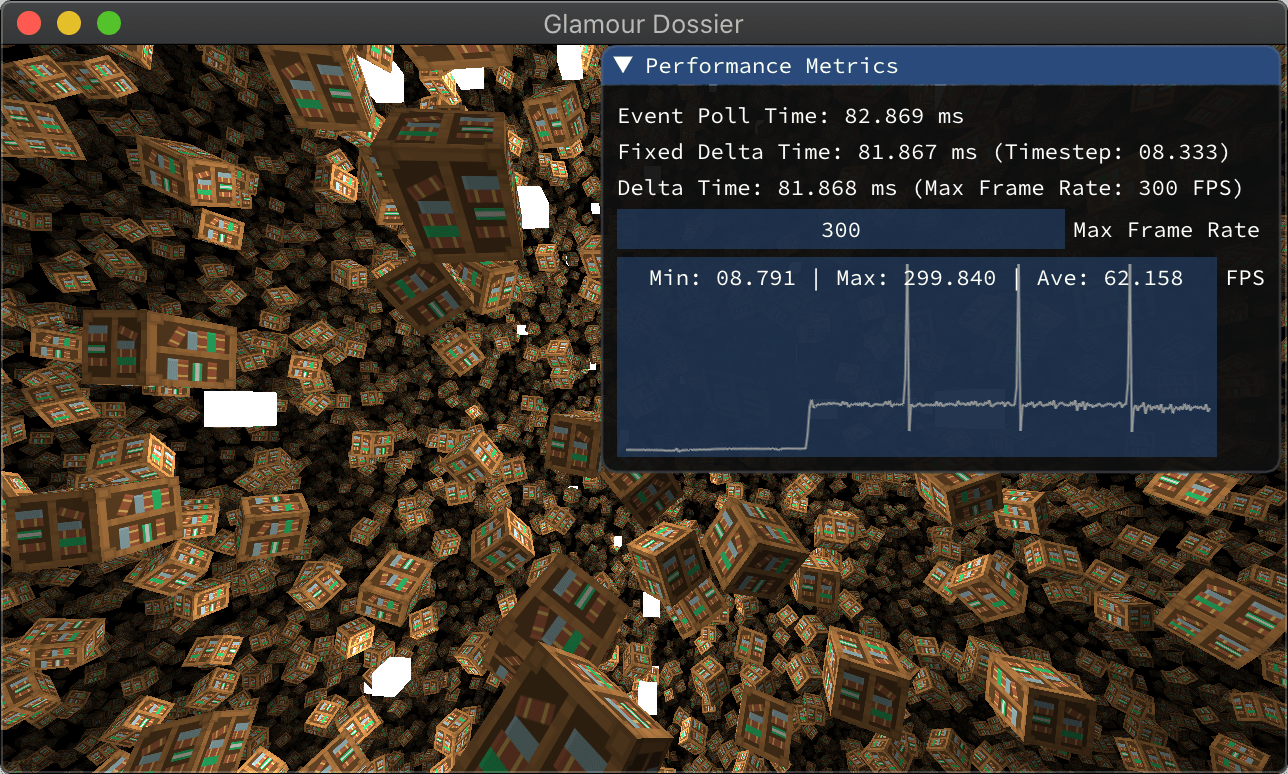
\includegraphics[width=0.6\columnwidth]{../app-screenshot.png}
  \end{center}
  \caption[Application Screenshot]{
    \emph{
      Running the application results in the scene above; many rotating textured cubes, with lights travelling around the world.
      Metrics provide real-time data about the performance.
    }
  }\label{fig:app-screenshot}
\end{figure}

\section{Method}
% - Restate question
%     - What is the measurable difference between forward/deferred?
% - Justify configuration
%     - How parameter changes help answer question
%     - What are my assumptions?
% - Configuration details
%     - Constants? But (small) why?
%     - Parameter sequence
%     - Ranges (appendix?)
%     - Example table
%         - Screenshot of test run

\subsection{Overview}
To find the measurable difference between the forward rendering and deferred rendering pipeline implementations in Glamour, several sets of parameters were configured, tested, measured, and modified to obtain a reasonable amount of data.
These parameters were all relevant to the goal of the research as they specifically targeted the data inputs where the rendering pipeline architectures differed.
Assuming that there were no other implementation details that affected the performance benchmarks in such a negative way, the testing configuration has resulted in accurate data.

\subsection{Configuration}
\paragraph{Constants.} There were a few constants throughout all test runs.
\begin{itemize}
  \item \textbf{Maximum Frame Rate} was 300 FPS, as an unlimited frame rate caused issues in testing
  \item \textbf{Warm Up Time} was 1 second; when parameters update, wait 1s before capturing data
  \item \textbf{Cube Positions} were between -100.0 and 100.0 in all three dimensions
  \item \textbf{Light Positions} were between -50.0 and 50.0 in all three dimensions
  \item \textbf{Camera Position} orbited with a 10.0 unit radius around the origin.
\end{itemize}

\paragraph{Parameters.} There were five parameters that made up each test run.
\begin{itemize}
  \item The length of time to run each test
  \item The resolution of the viewport
  \item The rendering pipeline to use
  \item The number of lights to simulate
  \item The number of cubes to simulate.
\end{itemize}

Specifically for lights and cubes, the increase in number was exponential for each step, to show any linearity in the data, see Table~\ref{tab:parameters}.
When the application was run, each unique combination of parameters was generated and iterated over.

\paragraph{The iteration was as follows:}
Each test case incremented the \textbf{Cubes} parameter to the next value, and repeated when it reaches the end.
Every five test cases (when \textbf{Cubes} repeated), the \textbf{Lights} parameter was incremented, and repeated similarly, so every 25 test cases.
The same pattern was followed with \textbf{Pipeline}, then \textbf{Resolution}, and finally \textbf{Time}.

That resulted in \(5 * 5 * 2 * 5 * 2 = 500\) test cases.
The tests were run on two different machines; a Dual Core MacBook with an integrated GPU, and a Quad Core Gaming Laptop with a discrete GPU. See Appendix~\ref{app:pc-spec}.
\\
\\
As an example, the test case with configuration number 69 was:
\begin{center}
  \begin{tabular}{r|l}
    \textbf{Time}       & 5s       \\
    \textbf{Resolution} & 1280×720 \\
    \textbf{Pipeline}   & Forward  \\
    \textbf{Lights}     & 177      \\
    \textbf{Cubes}      & 9456
  \end{tabular}
\end{center}
Which resulted in the output shown in Figure~\ref{fig:test-69}.

\begin{figure}[h!]
  \begin{center}
    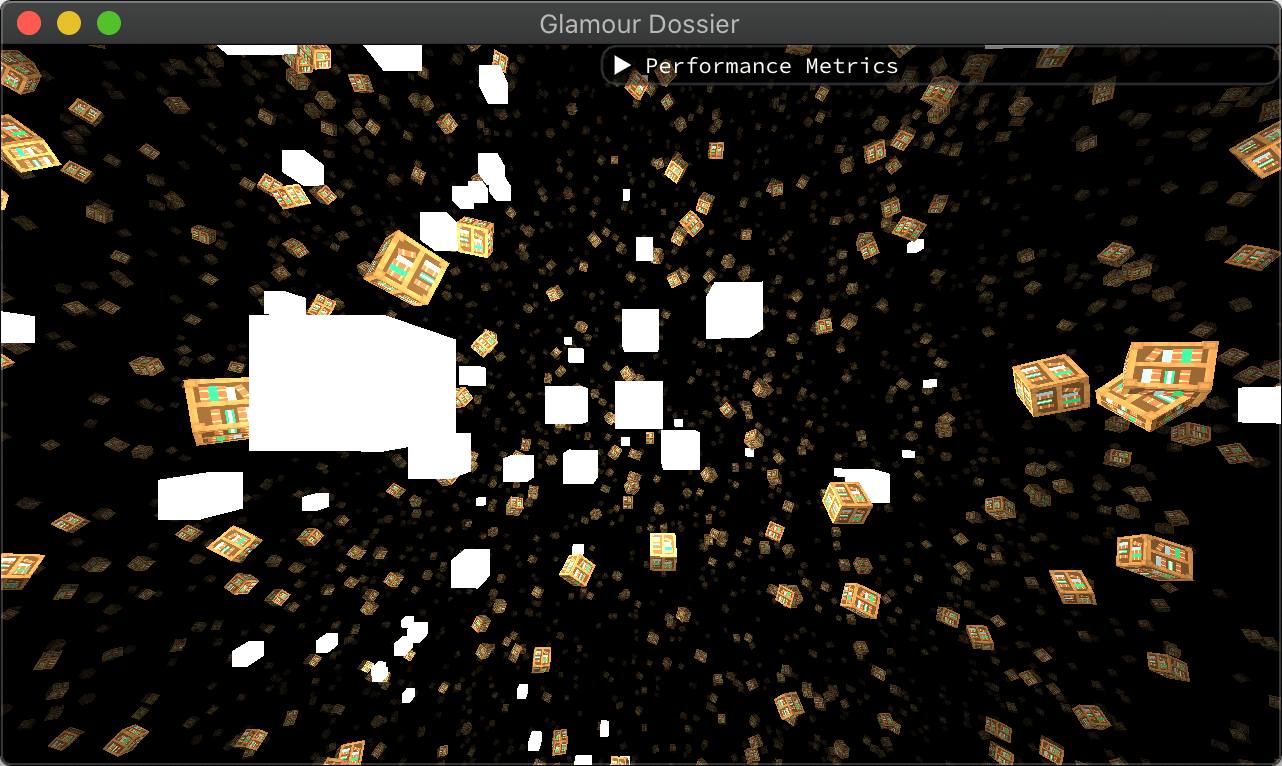
\includegraphics[width=0.6\columnwidth]{../test-69.png}
  \end{center}
  \caption[Test 69]{
    \emph{
      177 lights and 9,456 cubes.
    }
  }\label{fig:test-69}
\end{figure}

\begin{table}
  \caption[Parameter Table]{
    \emph{
      The parameters and each of their possible values.
      \textbf{Lights} and \textbf{Cubes} increase exponentially.
    }
  }\label{tab:parameters}
  \begin{center}
    \begin{tabular}{rlllll}
      \textbf{Time}       & 5s      & 20s      &           &           &           \\ \hline
      \textbf{Resolution} & 640×360 & 1280×720 & 1920×1080 & 2560×1440 & 3840×2160 \\ \hline
      \textbf{Pipeline}   & Forward & Deferred &           &           &           \\ \hline
      \textbf{Lights}     & 0       & 5        & 31        & 177       & 1,000     \\ \hline
      \textbf{Cubes}      & 0       & 20       & 446       & 9456      & 200,000
    \end{tabular}
  \end{center}
\end{table}


\section{Results}
% - Results (facts/data)
%     - Small words on data.
%         - Answer the question(s)
%         - Empirical evidence
%         - No speculation, only observation
%     - MEGA CHART (landscape)
%     - Other charts, e.g.
%         - Variation from avg
%     - Full data table in appendices

\subsection{Forward v Deferred}
With forward rendering, the performance can be seen as a multiplication of the cube count and light count.
With deferred rendering, the performance is more of an addition of the cube count and light count.
This is visible in Figure~\ref{fig:deferred-1080p-mac}; there is more of a linear increase in frame time as the light count increases.
Compared to Figure~\ref{fig:forward-1080p-mac}, where there is a saw-tooth effect happening as the cube count and light count are multiplied together.

This causes the performance to diverge greatly at high cube and light counts.
At the final configuration of each plot, with 200,000 cubes and 1,000 lights, the average frame time is about 500ms for deferred rendering but over three times that for forward rendering as it nears 2,000ms.

\begin{figure}[h!]
  \begin{center}
    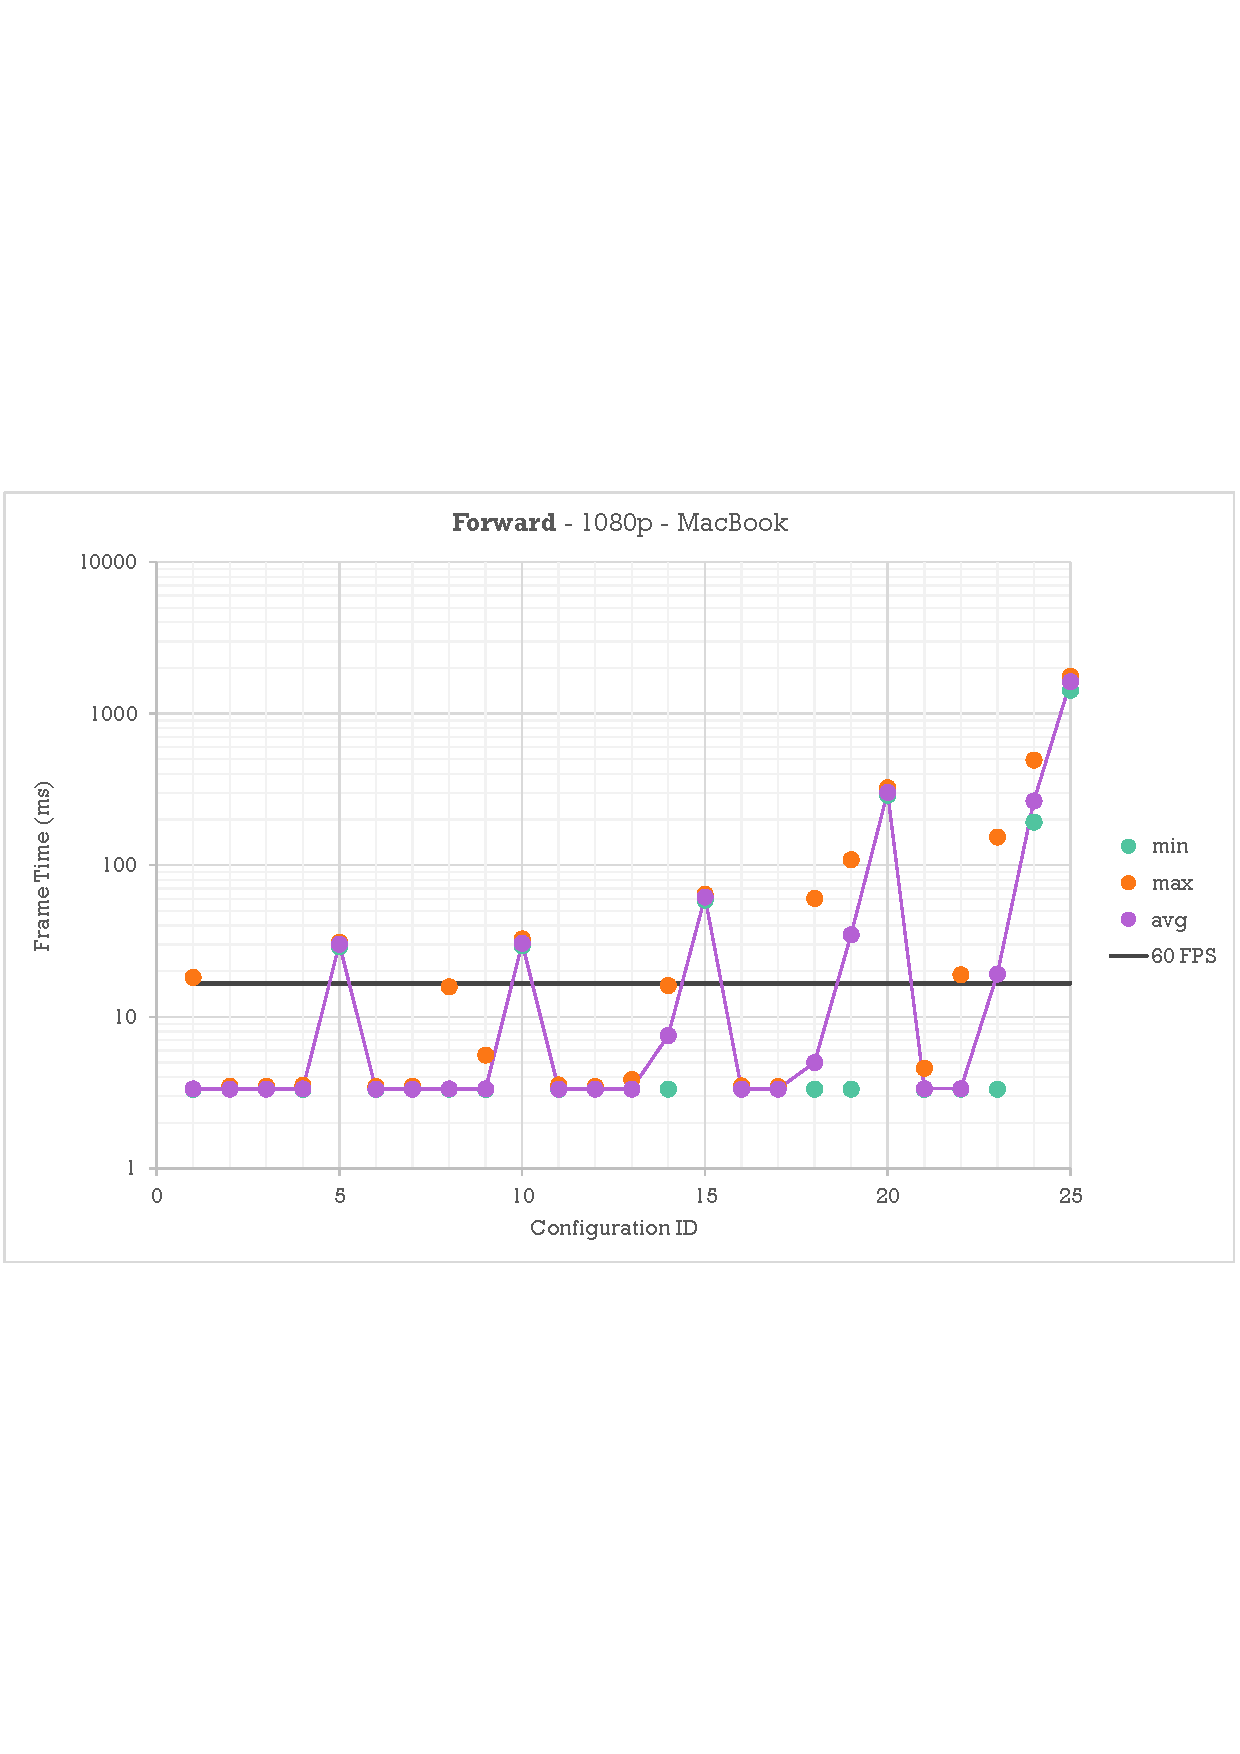
\includegraphics[width=1\columnwidth]{../forward-1080p-mac.pdf}
  \end{center}
  \caption[Forward 1080p]{
    \emph{
      Forward Rendering at 1920×1080 on the MacBook for 5s.
      Every configuration the cube count increases exponentially and repeats after 200,000.
      Every five configurations the light count increases exponentially up to 1,000.
      The frame time is measured in milliseconds with a logarithmic scale.
    }
  }\label{fig:forward-1080p-mac}
\end{figure}

\begin{figure}[h!]
  \begin{center}
    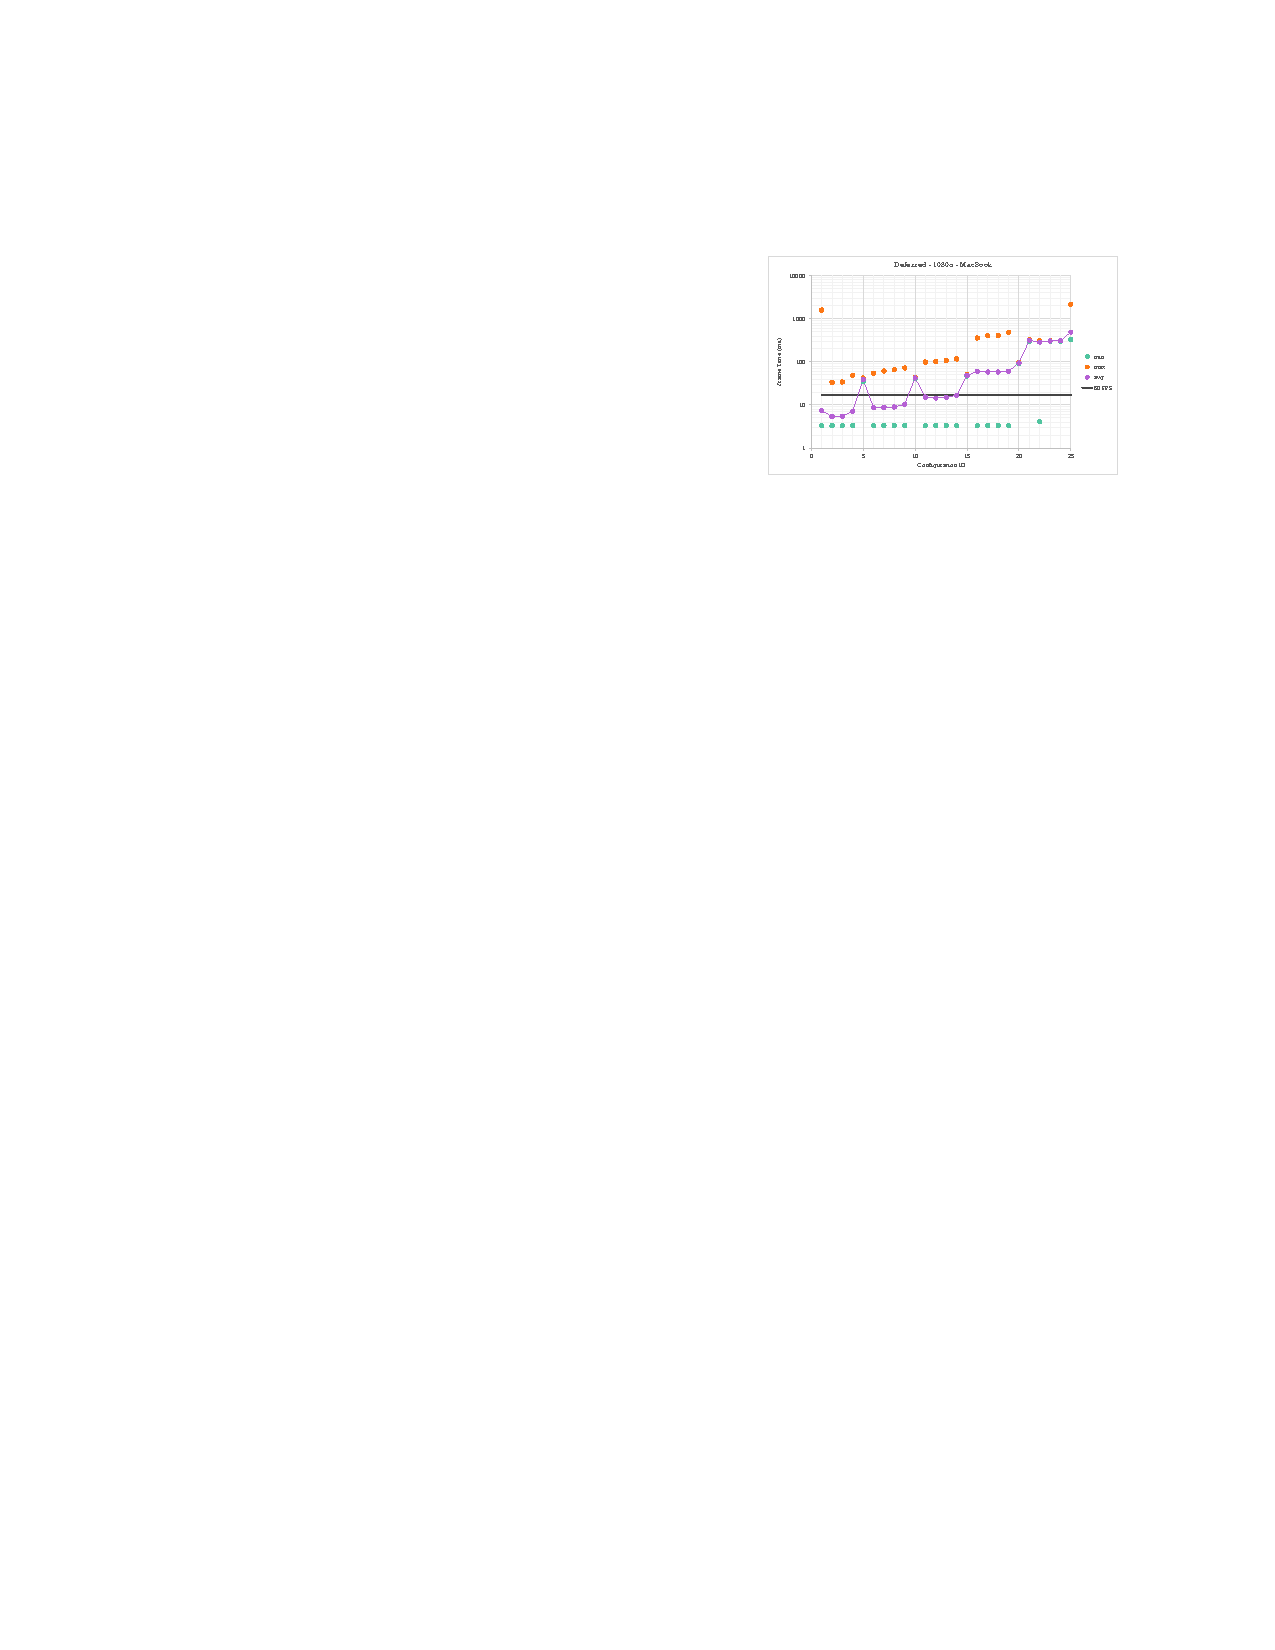
\includegraphics[width=1\columnwidth]{../deferred-1080p-mac.pdf}
  \end{center}
  \caption[Deferred 1080p]{
    \emph{
      Deferred Rendering at 1920×1080 on the MacBook for 5s.
      Every configuration the cube count increases exponentially and repeats after 200,000.
      Every five configurations the light count increases exponentially up to 1,000.
      The frame time is measured in milliseconds with a logarithmic scale.
    }
  }\label{fig:deferred-1080p-mac}
\end{figure}

\subsection{Comparing Resolutions}
In Figure~\ref{fig:mac-5s} it can be seen that the same performance pattern is repeated from Figures~\ref{fig:forward-1080p-mac} and~\ref{fig:deferred-1080p-mac} across multiple resolutions.
Each spike in the average frame time is still when there are 200,000 cubes being simulated.
The maximum frame time for deferred is often very similar to forward, however the average is generally much lower.

Also, there were multiple unprecedented issues experienced when running the test suite on the MacBook at the two highest resolutions (2560×1440 and 3840×2160).
The data could not be obtained, so it is not shown.

\begin{figure}[h!]
  \begin{center}
    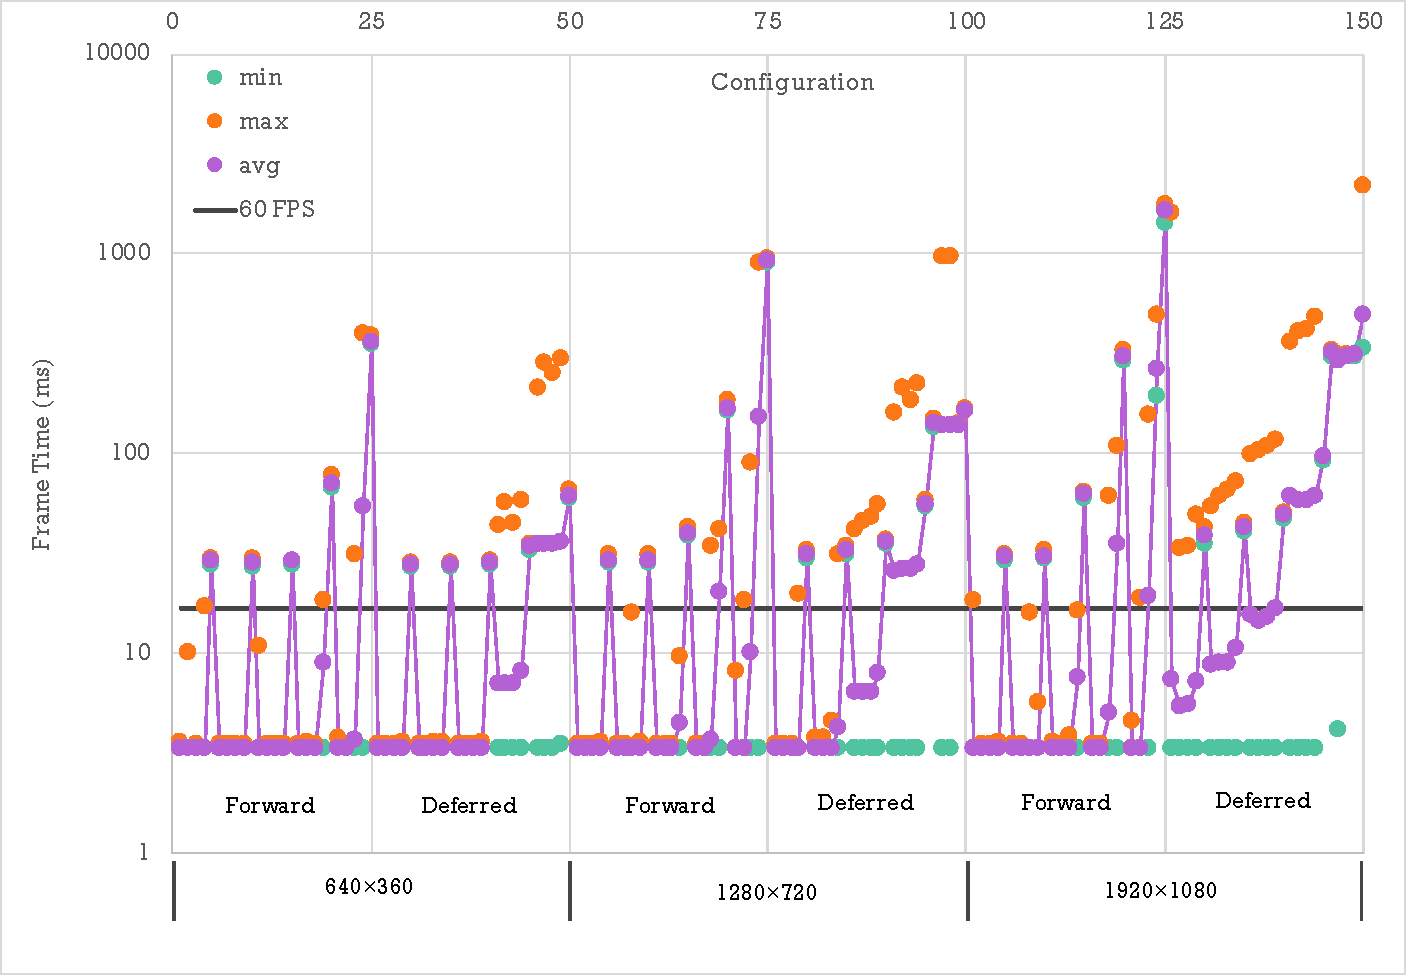
\includegraphics[width=1\columnwidth]{../mac-5s.pdf}
  \end{center}
  \caption[MacBook Data]{
    \emph{
      MacBook data with a 5s collection time.
      There was little to no difference between collection times of 5s and 20s.
      The minimums were just a little lower, and the maximums just a little higher.
    }
  }\label{fig:mac-5s}
\end{figure}

\subsection{Comparing Hardware}
Figure~\ref{fig:win-20s} shows the data for the Gaming Laptop running Windows.
The results follow similar trends to the MacBook data.
For example, Average frame time of the final configuration for forward and deferred pipelines is 2,261ms and 365ms respectively.
This is a similar magnitude of divergence in performance as the MacBook data.
However, minimum and maximum frame times are generally closer to the average compared to the MacBook results.

Interestingly, frame times for configurations 1 to 100 tightly surround 16.6 ms (60 FPS).
Configurations above 100 appear to bottom out at the set maximum frame rate of 300 FPS (3.3 ms)

\begin{figure}[h!]
  \begin{center}
    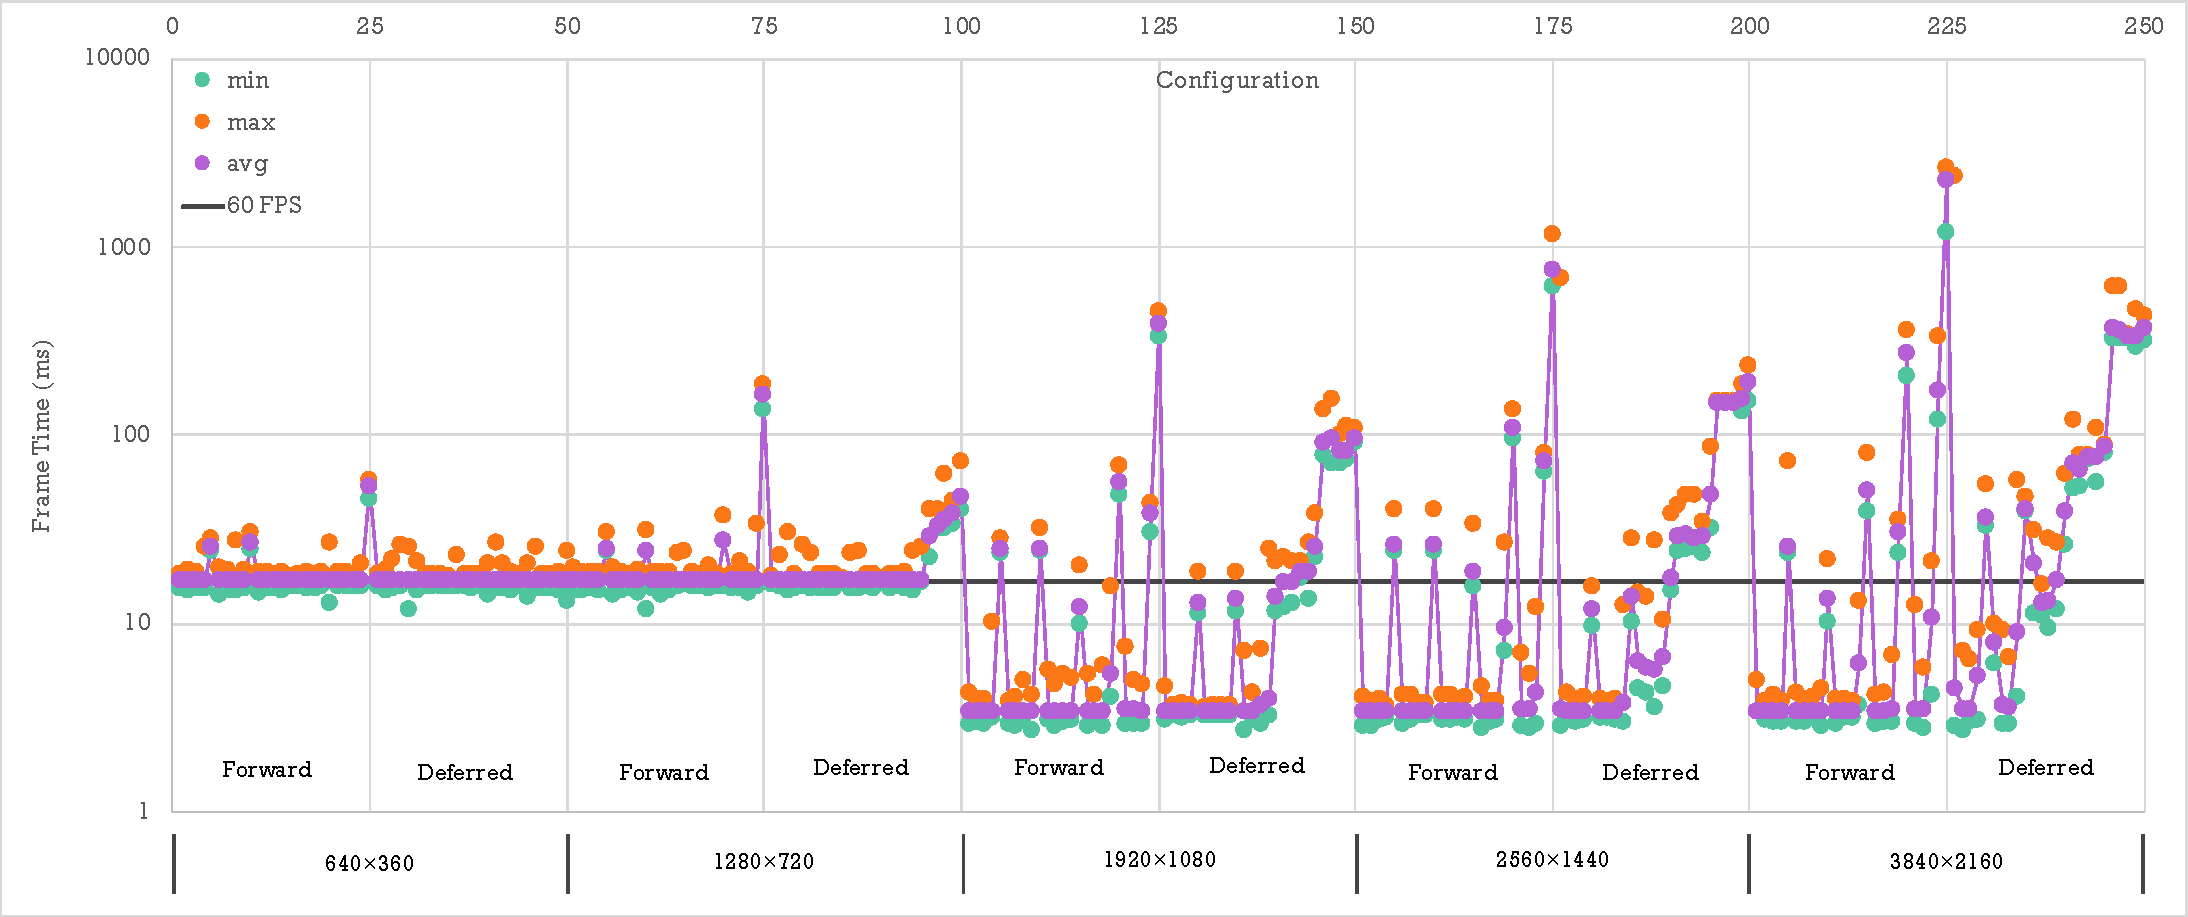
\includegraphics[width=1\columnwidth]{../win-20s.pdf}
  \end{center}
  \caption[Gaming Laptop Data]{
    \emph{
      Gaming Laptop data with a 20s collection time.
      Frame times are much lower compared to the MacBook when the light count and cube count is high.
    }
  }\label{fig:win-20s}
\end{figure}

\subsection{Overall}
The data show that forward rendering performs as good or better than deferred rendering when there are is a maximum of 446 cubes, no matter the number of lights.
If the cube count is higher than 446 and the light count is higher than 31, then deferred rendering performs better.
Deferred rendering keeps performing better as the cube count, light count, and resolution increase.

\section{Discussion}
% - Discussion (opinions)
%     - About Data
%     - About method
%     - About THE FUTURE
%         - Backlog teuxdeux list

\subsection{The Data}

The results were about what I expected.
As the number of cubes, lights, and the resolution increases, deferred rendering becomes the better choice.
This is not surprising, as the fundamental difference of deferred rendering is the dimensional reduction in shading complexity from rasterising the geometry so that lighting calculations only consider light count and resolution.

The overhead of deferred rendering is only observable at the higher resolutions (1080p for MacBook, 4K for Gaming Laptop).
This is most likely because of the addition of several frame buffers required for rasterising the geometry.
Since those frame buffers are screen-sized textures, the cost is greater for higher resolutions.
However, unless the scene is particularly basic, minimal geometry and lights, the cost is negligible.

Even though the rendering implementation is fairly rudimentary, there is still a measurable difference in the performance of forward rendering and deferred rendering.
This was very nice to see at this fundamental stage, and with improvements to the rendering process and data capture, the results can only become more significant.

\subsection{The Method}

\paragraph{The problem with frame time.}
Frame time is measured by the CPU and covers the entire application loop.
This is not the best measurement for comparing rendering performance, as the actual GPU time is lumped in with all the other artefacts.
However, it is useful to show that even if the GPU could render a scene efficiently, it might be totally infeasible to process that scene data through the CPU in the first place, making the rendering comparisons insignificant.
It would be nice to see at least a separation of CPU time and GPU time.

\paragraph{Lots of minimums.}
Throughout the data, a lot of the sample's minimum, maximum, and average are all ostensibly at 3.3ms (300 FPS).
Especially with the scale of the charts, the earlier samples are not useful for making comparisons with.
Running the application with a lower minimum frame time may have produced more accurate results.

\paragraph{Gaming Laptop samples.}
In the Gaming Laptop data, there are unusual samples from the first 100 configurations.
All the data points are around 60 FPS\@.
I believe this has something to do with the screen that those 100 tests were run on.
They were run on the laptop's internal display, whereas the proceeding tests were run on a 4K external display.
Both displays are 60Hz, the application had V-Sync disabled, but the internal laptop display has Nvidia G-Sync technology, which appeared to sync up the GPU frame rate with the internal screen's refresh rate.

\paragraph{GPU frame profiling.}
This is something that was planned, but the method of obtaining such information is arduous.
It would be interesting to sample an average frame from one of the test configurations and provide and visual and timed breakdown of the shader programs being run.
This extra data would show performance metrics for each part of the deep GPU pipeline.
Of which, could be used to aid in optimising the renderer.

\subsection{The Future}

\paragraph{Tiles and clusters.}
There are a few methods of optimising the shading complexity of a rendering pipeline, forward or deferred.
Tiling involves determining what pixels would be affected by what lights, and only sending those lights' details to the shader, thus reducing the lighting calculations for less lit parts of the screen.
Clustering has the same goal, but operates in 3D space to reduce lighting calculations even further under certain conditions\cite{olsson_clustered_2012}.

\paragraph{Complex geometry.}
Texture cubes are okay, but they're not the most difficult thing for a GPU to instance, and it's unlikely a game would only be rendering 200,000 of the same object.
Using real-world models, meshes, and materials would provide more practical information.

\paragraph{Interactive learning tool.}
Having gone through the effort of learning and building a rendering engine, I would have very much appreciated something to help me understand the implications of the pipelines, and 3D graphics as a whole.
It would be interesting to enhance this research tool to help others learn about computer graphics and test their knowledge or skills and compare it to other learning resources available.

\section{Conclusion}
% - Conclusion
%     - No new, only restate (dog meme)
%     - Emphasise the main outcome/implication

Forward rendering is a simple pipeline for basic scenes, but as the number of lights enters the hundreds and the scene's geometry becomes more complex, deferred rendering provides more consistent performance.

\section{Acknowledgements}

\paragraph{Clinton and Charlotte for supervising.}
Both of them were immeasurably helpful and supportive in providing me with the knowledge and resources to help me complete this research project.
Thank you. \emoji{🙏}

\paragraph{Joey de Vries of learnopengl.com}
I would have not been able to understand any 3D computer graphics without Joey's incredible series of tutorials.

\paragraph{Yan Chernikov of The Cherno.}
The Cherno has some excellent videos on OpenGL and game engine programming.
I like them. \emoji{👍}

\paragraph{The Rust community.}
My entire experience with Rust has been fantastic.
I just really dig the whole vibe that language and its community emits.

\newpage

%----------------------------------------------------------------------------------------
%	BIBLIOGRAPHY
%----------------------------------------------------------------------------------------

\printbibliography[heading=bibintoc]{}

\newpage

%----------------------------------------------------------------------------------------
%	APPENDICES
%----------------------------------------------------------------------------------------

\begin{appendices}

  \section{Computer Specifications}\label{app:pc-spec}

  \begin{table}[h!]
    \begin{tabular}{rl}
      \textbf{Device} & MacBook Pro (13-inch, 2017, Two Thunderbolt 3 ports) \\ \hline
      \textbf{CPU}    & Dual-Core Intel Core i5, 2.3 GHz                     \\ \hline
      \textbf{RAM}    & 8 GB                                                 \\ \hline
      \textbf{GPU}    & Intel Iris Plus Graphics 640, 1536 MB
    \end{tabular}
  \end{table}

  \begin{table}[h!]
    \begin{tabular}{rl}
      \textbf{Device} & Metabox P65xRP                   \\ \hline
      \textbf{CPU}    & Quad-Core Intel Core i7, 2.6 GHz \\ \hline
      \textbf{RAM}    & 16 GB                            \\ \hline
      \textbf{GPU}    & Nvidia GeForce GTX 1060, 6GB
    \end{tabular}
  \end{table}

\end{appendices}

\end{document}
